\begin{figure}[p]
\centering
    \begin{subfigure}[t]{0.45\textwidth}
    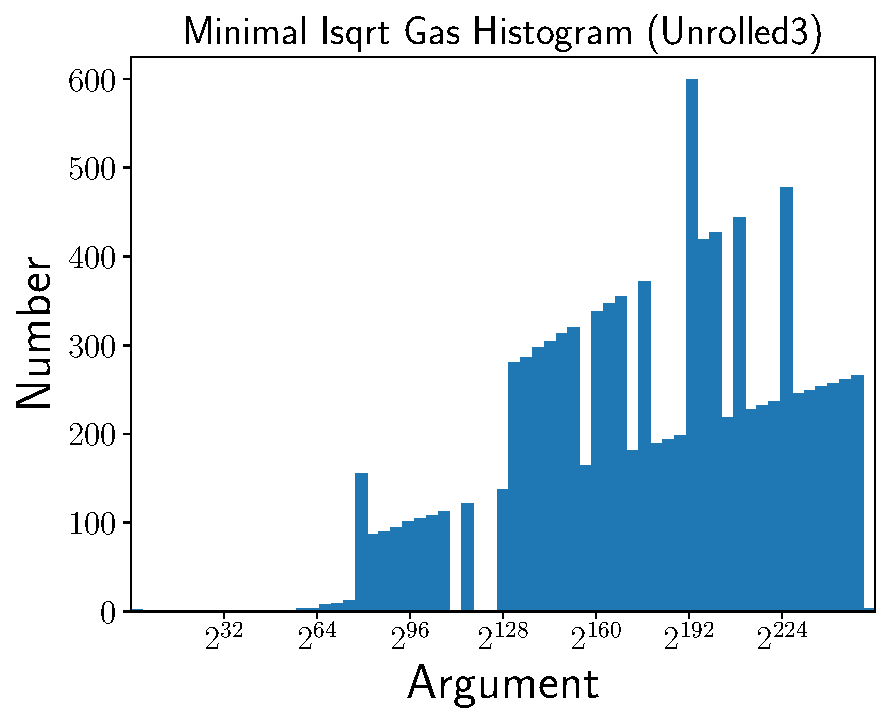
\includegraphics[width=\textwidth]{plots/minimal_hist_Unrolled3_ed.pdf}
    \end{subfigure}
    \begin{subfigure}[t]{0.45\textwidth}
    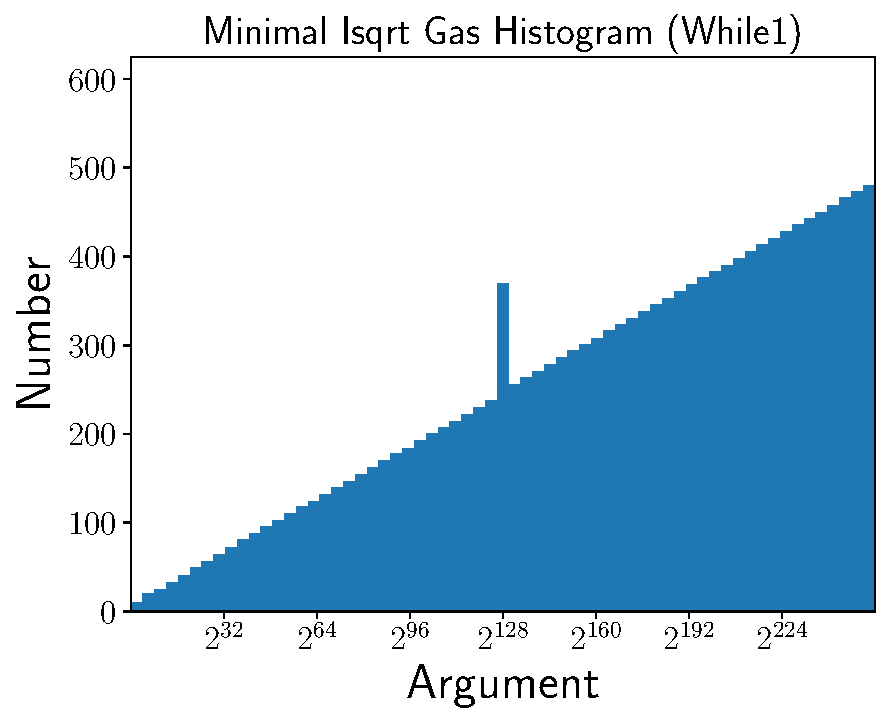
\includegraphics[width=\textwidth]{plots/minimal_hist_While1_ed.pdf}
    \end{subfigure}

    \begin{subfigure}[t]{0.45\textwidth}
    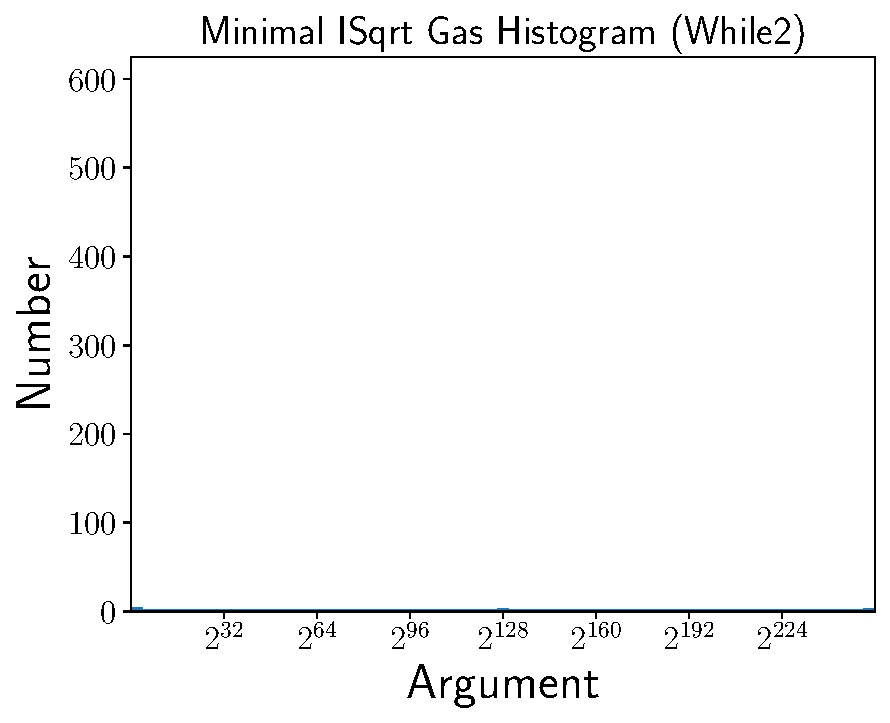
\includegraphics[width=\textwidth]{plots/minimal_hist_While2_ed.pdf}
    \end{subfigure}
    \begin{subfigure}[t]{0.45\textwidth}
    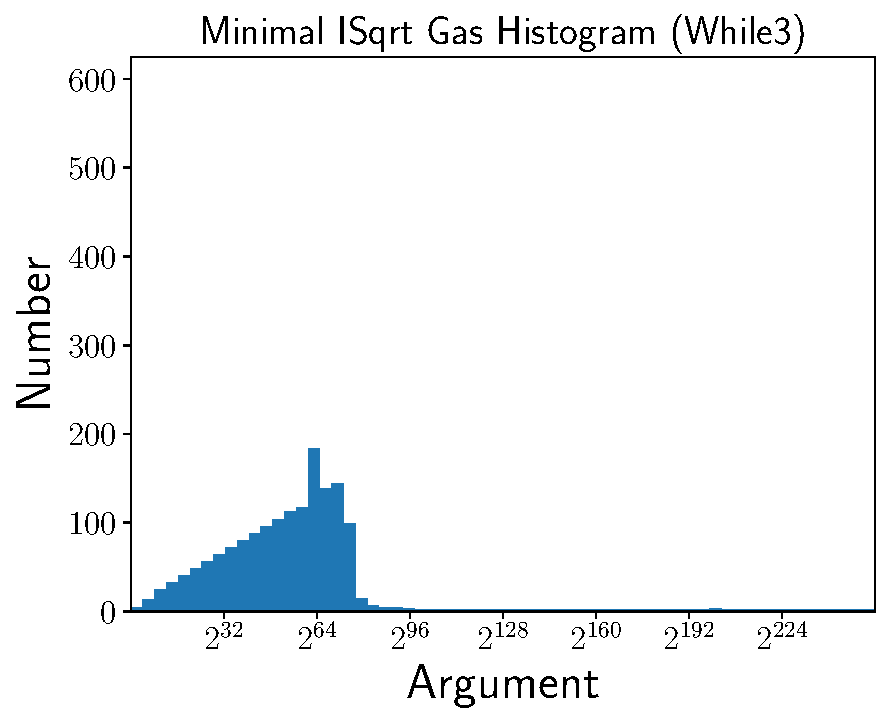
\includegraphics[width=\textwidth]{plots/minimal_hist_While3_ed.pdf}
    \end{subfigure}
    \caption{Here we plot a histogram showing where each algorithm is minimal
        when using a larger sample of deterministic values.
        Each bin counts the total number of instances where the algorithm's
        gas cost is minimal.
        These results are for the tests in Appendix~\ref{app:deterministic}.
        }
    \label{fig:minimal_gas_hist_ed}
\end{figure}
